%
% This document is available under the Creative Commons Attribution-ShareAlike
% License; additional terms may apply. See
%   * http://creativecommons.org/licenses/by-sa/3.0/
%   * http://creativecommons.org/licenses/by-sa/3.0/legalcode
%
% Created: 2011-08-14 17:43:38+02:00
% Main authors:
%     - Jérôme Pouiller <jezz@sysmic.org>
%

\tikzstyle{main}     = [node distance=1cm, transform shape, inner sep=0pt, outer sep=0pt, rounded corners=2mm, text centered, minimum height=0.9cm]
\tikzstyle{cred}     = [fill=red!20!white,     draw=red!50!black,     rounded corners=2mm]
\tikzstyle{cblue}    = [fill=blue!20!white,    draw=blue!50!black,    rounded corners=2mm]
\tikzstyle{cgreen}   = [fill=green!20!white,   draw=green!50!black,   rounded corners=2mm]
\tikzstyle{corange}  = [fill=orange!20!white,  draw=orange!50!black,  rounded corners=2mm]
\tikzstyle{cyellow}  = [fill=yellow!20!white,  draw=yellow!50!black,  rounded corners=2mm]
\tikzstyle{ccyan}    = [fill=cyan!20!white,    draw=cyan!50!black,    rounded corners=2mm]
\tikzstyle{cbrown}   = [fill=brown!20!white,   draw=brown!50!black,   rounded corners=2mm]
\tikzstyle{cpurple}  = [fill=purple!20!white,  draw=purple!50!black,  rounded corners=2mm]
\tikzstyle{size1}=[main, minimum width=1.9cm, text width=1.8cm]
\tikzstyle{size2}=[main, minimum width=3.9cm, text width=3.8cm]
\tikzstyle{size3}=[main, minimum width=5.9cm, text width=5.8cm]
\tikzstyle{size4}=[main, minimum width=7.9cm, text width=7.8cm]

\part{Linux et le temps réel}

\begin{frame}
\partpage
\end{frame}

\begin{frame}
\tableofcontents
\end{frame}

% \begin{frame}{Contexte}
%   Garantie qu'une action est éxecutée en moins d'un temps donné.

%   Implique:
%   \begin{itemize}
%     \item Une garantie de qualité (0 bug)
%     \item  Souvent  des processus  garantissant  la  qualité dans  les
%       différentes phases: conception, développement, validation
%     \item  Une connaissances  importante de  l'environnement extérieur
%       (fréquence maximum des interruption, etc...)
%   \end{itemize}
%   $\to$ On se limitera à l'architecture logicielle
% \end{frame}


% Schema des temps de réponses
% La principale chose que nous allons combattre, sera le temps de réponse aux
% évènements. Le temps de réponse peut-être très aléatoire
% Si on avait un temps de réponse null (ou au moins constant). Alors, il
% deviendrait simple de calculer les temps de réponse maximum de nos taches


\section{Problématique des OS RT} %(45min)

\begin{frame}{Limites des système classiques}
  Les systèmes classiques s'appuient  sur un système d'exploitation en
  général mal adapté pour le temps réel:
  \begin{itemize}
  \item Politique d'ordonnancement visant à équilibrer équitablement le
    temps alloué à chaque tâche
  \item La gestion de la  mémoire virtuelle, des caches engendrent des
    fluctuations temporelles
  \item La  gestion des temporisateurs  qui servent à  la manipulation
    des temps pas assez fin
  \item   Mécanismes   d'accès   aux   ressources  partagées   et   de
    synchronisation comportent des incertitudes temporelles
  \item Gestion des interruptions non-optimisées
  \item Systèmes non-certifiés
  \item API mal adaptées au systèmes temps réels
  \end{itemize}
\end{frame}

\section{Latences}

\begin{frame}{Latence aux évènements}
  \begin{itemize}
    \item Coeur du problème
    \item Si la latence était  nul (ou au moins constante), on calculerait
      simplement le temps de réponses de nos tâches.
  \end{itemize}

  \begin{center}
       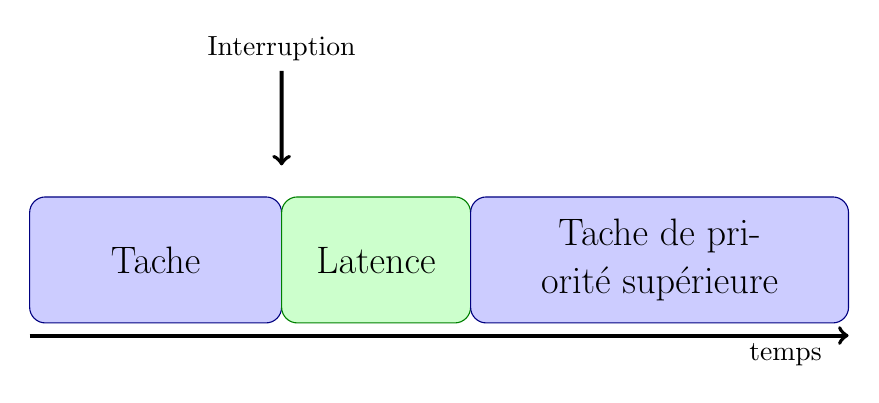
\begin{tikzpicture}[scale=0.8]
     \tikzstyle{msize}=[main, minimum height=2cm, font=\LARGE]
     \draw
       node[anchor=south]                at (2, 3) {Interruption}
       edge[->, line width=0.5mm]  (2, 1.5)
       node[msize, cblue,  minimum width=4cm, text width=4cm] at (  0, 0) {Tache}
       node[msize, cgreen, minimum width=3cm, text width=3cm] at (3.5, 0) {Latence}
       node[msize, cblue,  minimum width=6cm, text width=6cm] at (  8, 0) {Tache de priorité supérieure}
       (-2, -1.2) edge[->, line width=0.5mm]  (11, -1.2)
       node at (10, -1.5) {temps};
   \end{tikzpicture}

  \end{center}
\end{frame}

\begin{frame}{Latence aux évènements}{Exemple concret}
  \begin{itemize}
  \item On paramètre un timer à 50Hz
  \item On mesure le temps effectif de chaque période
  \end{itemize}
  \begin{center}
    \pgfimage[width=10cm]{pics/blachier_1}
  \end{center}
\end{frame}

% Exemple concret
% Expliquer que l'on paramètre un timer à 50Hz
% On mesure les période effectives
% Le temps de réponse est ici très aléatoire et dépend fortement de la charge de la machine
% Schema des temps de réponses
\begin{frame}{Latence aux évènements}{Système temps réel}
  \begin{center}
    \pgfimage[width=10cm]{pics/blachier_3}
  \end{center}
\end{frame}

% Le temps de réponse ici est beaucoup mieux borné
% Schema des temps de réponses
\begin{frame}{Latence aux évènements}{Système temps réels}
  \begin{center}
    \pgfimage[width=10cm]{pics/latencyRT}
  \end{center}
\end{frame}

\begin{frame}{Latence aux évènements}{Système classique}
  \begin{center}
    \pgfimage[width=10cm]{pics/blachier_4}
  \end{center}
\end{frame}

\begin{frame}{Latence aux évènements}{Système classique}
  \begin{center}
    \pgfimage[width=10cm]{pics/latencyNorm}
  \end{center}
\end{frame}

%     -> Taches RT << 100\%
%     ->  --> Algorithme d'ordonnancement secondaire (RM vs EDF)
%     -> Rendre cette formule assez simple pour être prédictible
%     %-> CAD limiter les effets des tache apériodique de priorité supérieure:
%        Interruptions, cache miss, changement de contexte, etc...
%     -> Présenter les diagramme normal va RT

\section{Bases}

\begin{frame}{Mécanisme basiques}
  \begin{itemize}
  \item  Possibilité  d'exécuter  une  tache avec  \c{SCHED_RT}  ou
    \c{SCHED_FIFO} (priorité toujours inférieure aux \emph{sofirqs} du noyau)
  \item Possibilité de marquer les pages de mémoire avec \c{mlock}
  \item L'accès  à des  horloges haute précision  est un  élément clef
    d'un système temps réel.
    \begin{itemize}
    \item Le framework  \emph{hpet} (\emph{High Precision Timers}) est
      assez récent dans le noyau Linux (2001) (à titre de comparaison,
      l'équivalent de \emph{hpet} est  apparu sous Windows à partir de
      Vista).
    \item Autrefois, l'horloge  était utilisée pour l'ordonnanceur. Le
      temps retourné  par les différents services  était celui calculé
      par l'ordonnanceur.   Avec \emph{hpet}, les  horloges sont des
      périphériques à part entière
    \end{itemize}
  \end{itemize}
\end{frame}

\begin{frame}{Contexte}
  Ordonnancement statique:
  \begin{itemize}
    \item Charge des taches temps réelles $\ll 100\%$
    \item[$\to$]   Ordonnancement   avec   des   priorités   statiques
      suffisante
    \item[$\to$]  Problématique  des  algorithmes  d'ordonnancement  à
      priorité dynamique (EDF, LST, etc...) secondaire
  \end{itemize}
\end{frame}

% % En d'autre termes:
% \begin{frame}{Contexte}
%   $$TR_i = C_i + \sum_{P_j > P_i} \left\lceil\frac{TR_i}{T_j}\right\rceil C_j$$
% Pour les allergiques: le temps de réponse d'une tâche est égal à la somme du
% temps d'exécution de la tache et de toutes les tâche de priorité supérieure
% qui s'exécutent en même temps.\\[1.5ex]
% Objectif: Rendre cette formule assez simple pour être prédictible.\\[1.5ex]
% Pas si simple:
%   \begin{itemize}
%     \item Interruptions
%     \item Changement de contexte
%     \item Sections critiques (ordonnanceur désactivé)
%     \item Caches, Swap
%   \end{itemize}
% \end{frame}

\section{Systèmes Symétriques et Asymétriques}

\begin{frame}{Architectures multi-coeurs}
  Il est  possible d'utiliser  des architecture multi-coeurs  pour des
  systèmes temps réels.
  \\
  On distingue alors 2 types d'architectures:
  \begin{itemize}
  \item  Les systèmes  symétriques (SMP)  où  les tâches  ne sont  pas
    affectées à un CPU particulier
  \item  Les  systèmes asymétriques  où  on  affecte manuellement  les
    tâches à un CPU
  \end{itemize}
\end{frame}

\begin{frame}{Systèmes asymétriques}
  Les systèmes asymétriques sont assez simples à architecturer:
  \begin{itemize}
  \item On effectue une étude séparées pour chaque CPU
  \item   On  considère  les   échanges  entre   les  CPU   comme  des
    entrées/sorties
  \end{itemize}
  Sous Linux, il  est possible d'associer une tâche  avec un CPU grâce
  à:
  \begin{itemize}
  \item la fonction \emph{CPU affinity}
  \item la commande \c{taskset} ou \c{lxc}
  \item aux fonctions \emph{cgroup} et \emph{cpuset}
  \end{itemize}
  \note{ca     fonctionne     avec     \texttt{mount     -t     cpuset
      /mnt/cpuset. cf. Documentation/cgroup/cpuset.txt}}
\end{frame}

\begin{frame}[fragile=singleslide]{LXC}
  \cmd{lxc} permet de créer des  container et d'avoir une gestion fine
  des limitations de ressources.
  \begin{itemize}
  \item Activer \emph{Control Group Support} dans le noyau
  \item Démonstration avec \file{lxc-test.c}
    \begin{lstlisting}
$ gcc samples/lxc-test.c -o lxc-test
$ apt-get install lxc
    \end{lstlisting}
  \item Création d'un container et éxecution de la commande
    \begin{lstlisting}
$ lxc-create -n test
$ lxc-execute -n test ./lxc-test
    \end{lstlisting}
  \end{itemize}
\end{frame}

\begin{frame}[fragile=singleslide]{LXC}
  \begin{itemize}
  \item Limiter le container à au CPU 0:
    \begin{lstlisting}
$ lxc-cgroup -n test cpuset.cpus 0
    \end{lstlisting}
  \item Supprimer la limite:
    \begin{lstlisting}
$ lxc-cgroup -n test cpuset.cpus 0,1
    \end{lstlisting}
  \item Limiter la consommation cpu à 10\%:
    \begin{lstlisting}
$ lxc-cgroup -n test cpu.cfs_quota_us 10000
    \end{lstlisting}
  \item Retirer la limite:
    \begin{lstlisting}
$ lxc-cgroup -n test cpu.cfs_quota_us -1
    \end{lstlisting}
  \item Connaitre la consommation CPU du container:
    \begin{lstlisting}
$ lxc-cgroup -n test cpuacct.usage
    \end{lstlisting}
  \item cf. \file{/sys/fs/cgroup/}
  \end{itemize}
\end{frame}

\begin{frame}{Systèmes symétriques}
  \begin{itemize}
  \item Beaucoup plus complexe à architecturer
  \item  La plupart de  nos algorithme  ne sont  plus prouvé  dans une
    architecture SMP
  \item La technologie est relativement récente (fin des années 90)
  \item Pourquoi si tard?
    \begin{itemize}
    \item Principalement problèmes matériels
    \item Problèmes de barrières mémoires (hard ou soft)
    \item Algorithme  beaucoup plus  ardu (inversion de  priorité par
      exemple)
    \end{itemize}
  \end{itemize}
\end{frame}

\begin{frame}{Temps réel dans le noyau}
  Travailler dans le noyau:
  \begin{itemize}
  \item Possibilité de travailler sous interruptions
  \item ... ou de travailler avec les soft IRQ et/ou les tasklets
  \item Oblige à travailler dans le noyau (problèmes d'APIs, etc...)
  \item Nécessaite beauoup de connaissance pour faire quelque chose de bien
  \item Accès  difficiles aux bibliothèques de haut  niveau (un simple
    accès au réseau peut devenir très complexe)
  \item  Gardez le  kernel  pour faire  des  drivers, externalisez  le
    traitement
  \end{itemize}
\end{frame}


\section{Low latency}

\begin{frame}{Noyau low latency}{Problème du noyau normal}
  Dans un  noyau Linux classique, il  y a un seul  contexte noyau pour
  tout le monde
  \begin{itemize}
  \item Pas possible de préempter le système
  \item Personne ne peut prendre  la main lorsqu'un processus est dans
    un \emph{syscall} (ordonnanceur désactivé)
  \item Équivalent d'une ressource partagée par tout les processus
  \item[$\to$] Latence
  \end{itemize}
\end{frame}

\begin{frame}{Noyau low latency}{Implémentation}
  \begin{itemize}
  \item Difficile de gérer les différents contextes noyau
  \item[$\to$] Noyau réentrant (= thread-safe)
  \item Gestion des interruption assez complexe
  \item Overhead assez important
  \end{itemize}
\end{frame}
%         -> Explique le problème des contexte noyaux
%         -> Définition de "Réentrant" (thread-safe)

\begin{frame}{Noyau low latency}{Résultats}
  \begin{itemize}
  \item Patch low-latency  mergé dans le mainstream avec  le noyau 2.6
    (\c{CONFIG_PREEMPT})
  \item Latences maximum de l'ordre de 300µs (chiffres de l'époque)
  \end{itemize}
\end{frame}

\section{Hyperviseurs}

\begin{frame}{Hyperviseur}
  \begin{itemize}
  \item Noyau low latency encore problématique pour les interruptions
  \item Beaucoup d'interruptions $\to$ latence
  \item Hyperviseur
  \end{itemize}
\end{frame}

\begin{frame}{Temps réel}{Nano Kernel}
  \begin{center}
    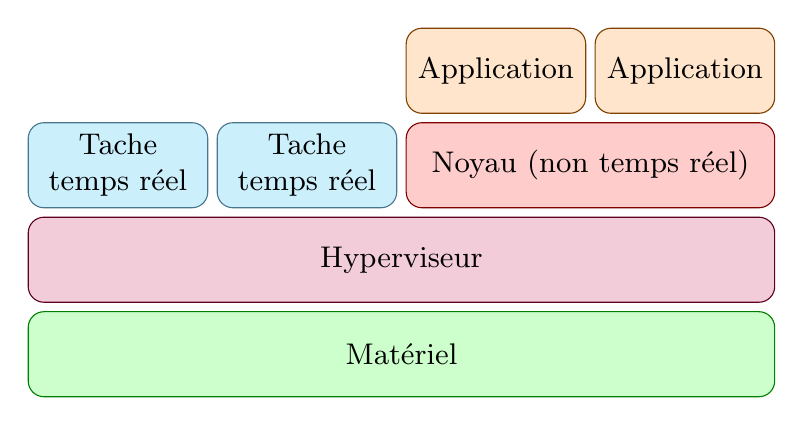
\begin{tikzpicture}[scale=1.2]
  \draw[font=\small]
    node[size1, ccyan]   at (1, 2) {Tache temps réel}
    node[size1, ccyan]   at (3, 2) {Tache temps réel}
    node[size1, corange] at (5, 3) {Application}
    node[size1, corange] at (7, 3) {Application}
    node[size2, cred]    at (6, 2) {Noyau (non temps réel)}
    node[size4, cpurple] at (4, 1) {Hyperviseur}
    node[size4, cgreen]  at (4, 0) {Matériel};
\end{tikzpicture}

  \end{center}
\end{frame}

\begin{frame}{Hyperviseur}
  \begin{itemize}
  \item Possibilité de préempter le noyau sans patch low-latency
  \item Possibilité de différer les interruptions
  \item  Possibilité  d'ignorer les  interruptions  dans les  sections
    temps réelles
  \item Performances excellentes (< 20µs)
  \item Technique non spécifique à Linux
  \item Peu de code en mode temps réel
  \item[$\to$] Certifiable

  \item Fonctionne au dessus du noyau
  \item Comportement des interruptions à modifier
  \item Communication entre les tâches temps réelles et le reste
  \item[$\to$] Nécessite de patcher le noyau
  \item           RTLinux,           RTAI           et           Adeos
    (\url{http://download.gna.org/adeos/patches/},
    \url{git://git.xenomai.org/ipipe-gch.git}) (Xenomai)
  \end{itemize}
\end{frame}

\begin{frame}{Hyperviseur}{Adeos}
  \begin{itemize}
    \item Fork de RTAI
    \item API utilisateur assurée par Xenomai
    \begin{itemize}
      \item Skins
      \item[$\to$]  Possibilité de  faire fonctionner  une application
        développée pour vxWorks
% Parler de vxWorks: Référence dans le domaine des OS RT Posix, OS des sondes Martiennes
      \item Skin native consistante
      \item Beaucoup mieux que Posix (de plus, il existe une skin Posix)
      \item \url{http://www.xenomai.org/documentation/xenomai-head/html/api}
    \end{itemize}
  \end{itemize}
\end{frame}

\begin{frame}[fragile=singleslide]{Adeos}
  Installation du patch noyau
  \begin{lstlisting}
$ wget https://xenomai.org/downloads/ipipe/v3.x/arm/older/ipipe-core-3.10.32-arm-9.patch
$ wget http://download.gna.org/xenomai/stable/xenomai-2.6.4.tar.bz2
$ tar xvf xenomai-2.6.4.tar.bz2
$ xenomai-2.6.4/scripts/prepare-kernel.sh --ipipe=ipipe-core-3.10.32-arm-9.patch --arch=arm --linux=linux-3.10.32
$ cd linux-3.10.32
$ make ARCH=arm menuconfig
$ make ARCH=arm uImage modules
$ sudo make INSTALL_MOD_PATH=/home/user/nfs ARCH=arm modules_install
$ sudo mknod /home/user/nfs/dev/rtheap c 10 254
$ sudo mknod /home/user/nfs/dev/rtscope c 10 253
$ sudo mknod /home/user/nfs/dev/rtp c 150 0
  \end{lstlisting}
\end{frame}

\begin{frame}[fragile=singleslide]{Adeos}
  Installation (Autotools classiques) de la bibliothèque Xenomai:
  \begin{lstlisting}
$ cd ../xenomai-2.6.4
$ ./configure --host=arm-linux --enable-shared=yes --enable-smp
$ make
$ sudo -E make DESTDIR=/home/user/nfs install
  \end{lstlisting}
  \begin{itemize}
  \item   Possibilité de faire la même chose avec Buildroot
  \item Il  sera ensuite nécessaire de compiler  les programme Xenomai
    avec le résultat de
    \begin{lstlisting}
$ xeno-config --skin=native --ldflags/--cflags | sed 's:=/:=/home/user/nfs/'
    \end{lstlisting}
  \end{itemize}
\end{frame}

\begin{frame}[fragile=singleslide]{Xenomai}
  Les choses intéressantes:
  \begin{itemize}
  \item Charger le système:
    \begin{lstlisting}
target# mount -t jffs2 /dev/mtdblock1 /mnt
target# /usr/xenomai/bin/dohell -m /mnt 10
    \end{lstlisting}
  \item Vérifier la latence d'une tâche périodique:
    \begin{lstlisting}
target# /usr/xenomai/bin/latency -t 0
    \end{lstlisting}
    Testons ensuite avec \c{-t 1} et \c{-t 2}
  \item Vérifier le temps de calcul sur des flottants:
    \begin{lstlisting}
target# /usr/xenomai/bin/arith
    \end{lstlisting}
    Les valeurs \emph{rejected}  ont eu un temps de calcul  > à 4 fois
    la moyenne (même si je ne  suis pas tout à fait d'accord avec leur
    manière de compter).
  \end{itemize}
\end{frame}

\section{RT-préempt} % (30min)

\begin{frame}{RT-preempt} % (15min)
  Gestion des interruption dans des threads
%     -> Rappeller vous de nos spin_lock
  \begin{itemize}
    \item Permet de préempter les interruptions
    \item[$\to$] Moins de latence des taches
    \item Permet d'ordonnancer les interruption
    \item[$\to$] Permet de se passer de la désactivation des interruptions
    \item[$\to$] Permet de remplacer les spin lock par des mutex
    \item[$\to$] Moins de latence des interruptions
  \end{itemize}
\end{frame}

\begin{frame}{RT-preempt}
  \begin{center}
    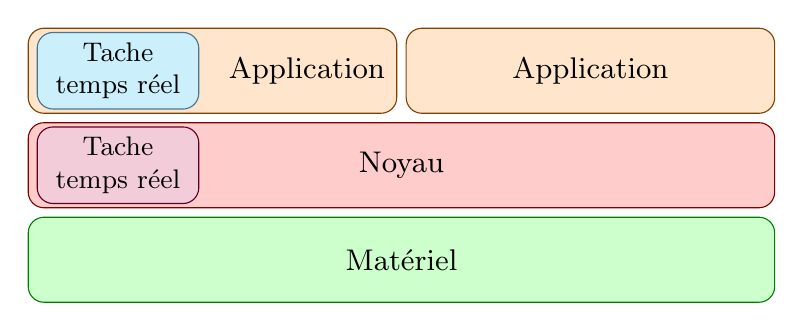
\begin{tikzpicture}[scale=1.2]
  \draw[font=\small]
    node[size2, corange]    at (6, 2) {Application}
    node[size2, corange]    at (2, 2) { } 
    node[size1]             at (3, 2) {Application}
    node[size1, ccyan, scale=0.9] at (1, 2) {Tache temps réel}
    node[size4, cred]       at (4, 1) { } 
    node[size3]             at (4, 1) {Noyau}
    node[size1, cpurple, scale=0.9] at (1, 1) {Tache temps réel}
    node[size4, cgreen]     at (4, 0) {Matériel};
\end{tikzpicture}

  \end{center}
\end{frame}

\begin{frame}{RT-preempt}
 \begin{itemize}
 \item                 Patch                RT                (Patchs:
   \url{http://www.kernel.org/pub/linux/kernel/projects/rt/},   Git:
   \url{git://git.kernel.org/pub/scm/linux/kernel/git/rostedt/linux-rt.git})
  \item Implémentation assez complexe
  \item[$\to$] Non portable
  \item Performance très bonnes (~20µs)
  \item Intégré en partie dans le noyau 3.0
 \end{itemize}
\end{frame}
%     -> Gère les interruption dans des thread
%     -> /!\ Pas portable partout
%     -> Implémentation assez tordue (c'est un cinglé qui a fait ca).
%     -> PatchRT
